\livelloA{Elementary Statistics}

\livelloB{Comparison of the postcards sales in two countries}

\begin{frame} 
\begin{description}
\item[Data:] cardsales.txt\\
Postcard sales data in the countries of New York and Florida day by day, from 1 January to 31 March.
\item[Aims:] \begin{itemize}
\item 
Let us numerically and graphically evaluate the distribution of the number of postcards sold in the two countries.
\begin{itemize}
\item[-] Which country has sold the most?
\item[-] Which country has more variability? 
\item[-] Are there anomalies?
\end{itemize}
\item Let us graphically check if the number of postcards sold daily in the two countries ``is associated '' somehow.
\end{itemize}

\end{description}
 
\end{frame}

%%%%%%%%%%%%%%%%%%%%%%%%%%%%%%%%%%%%%%%%%%%%%%%%%%%%%%%%%%%%%%%
\begin{frame}
Computation of descriptive statistics and B-W graphic:\\
	\vspace{.3cm}
	\begin{footnotesize}
	\begin{tabular}{|l|rrrrrrr|}
	\hline
	& \textbf{Min}. & 1\textbf{st.Qu}. & \textbf{Median} & \textbf{Mean} & \textbf{3rd.Qu.} & \textbf{Max.} & \textbf{Sd}\\
	\hline
	\textbf{FL.Sales (N=91)} & 1420 & 1484 & 1514 & 1514 & 1544 & 1640 & 46.52 \\
	\textbf{NY.Sales (N=91)} & 0 & 1654 & 1687 & 1671 & 1720 & 1813 & 183.65 \\
	\hline	
	\end{tabular}
	\end{footnotesize}
	\begin{center}
		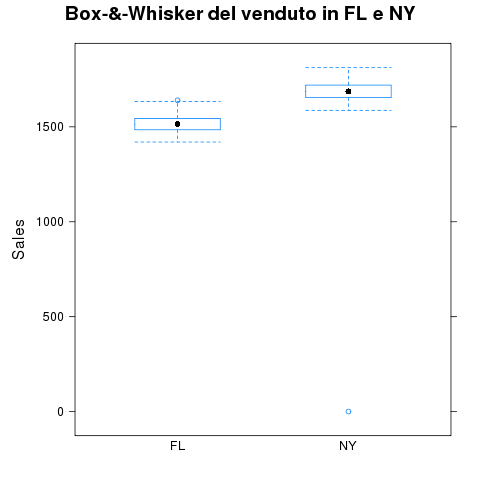
\includegraphics[width=6cm]{14_1.png}
	\end{center}
\end{frame}


%%%%%%%%%%%%%%%%%%%%%%%%%%%%%%%%%%%%%%%%%%%%%%%%%%%%%%%%%%%%%%%
\begin{frame}
\begin{itemize}
 \item Both the mean and the standard deviation of the sold in New York are greater than the respective statistics of the sold in Florida.
 \item It is necessary to note that the sold in New York has at least one day with 0 cards.
 \item Analysing the data, It is possible to understand that the day 20 of January, 0 postcards have been sold in New York because of a strike.
 \item That value will be removed to analyse again the data, in order to understand if the differences are still as relevant. 
\end{itemize}

\end{frame}

%%%%%%%%%%%%%%%%%%%%%%%%%%%%%%%%%%%%%%%%%%%%%%%%%%%%%%%%%%%%%%%
\begin{frame}
Computation of descriptive statistics and B-W graphic: (0 of NY deleted):\\
	\vspace{.3cm}
	\begin{footnotesize}
	\begin{tabular}{|l|rrrrrrr|}
	\hline
	& \textbf{Min.} & \textbf{1st.Qu.} & \textbf{Median} & \textbf{Mean} & \textbf{3rd.Qu.} & \textbf{Max.} & \textbf{Sd}\\
	\hline
	\textbf{FL.Sales (N=91)} & 1420 & 1484 & 1514 & 1514 & 1544 & 1640  & 46.52 \\
	\textbf{NY.Sales (N=90)} & 1587 & 1656 & 1687 & 1690 & 1721 & 1813 & 48.65 \\
	\hline	
	\end{tabular}
	\end{footnotesize}
	\begin{center}
		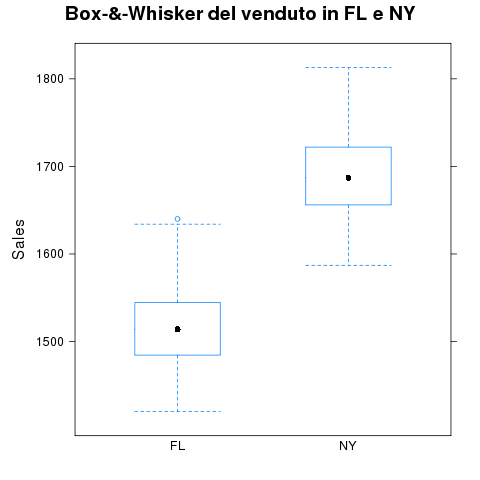
\includegraphics[width=6cm]{14_2.png}
	\end{center}
\end{frame}

%%%%%%%%%%%%%%%%%%%%%%%%%%%%%%%%%%%%%%%%%%%%%%%%%%%%%%%%%%%%%%%
\begin{frame}
\begin{itemize}
 \item The elimination of the 0 value has changed much the values of the statistics for only New York.
 \item Mean and median of the number of postcards sold daily are greater for New York.
 \item Indeed, New York has a number of postcards sold daily almost always higher than the Florida.
 \item The dispersion in the two countries is very similar.
 \item The distribution of the number of postcards sold, in general, seems to differ only for location.
\end{itemize}

\end{frame}

%%%%%%%%%%%%%%%%%%%%%%%%%%%%%%%%%%%%%%%%%%%%%%%%%%%%%%%%%%%%%%%
\begin{frame}
	\begin{center}
		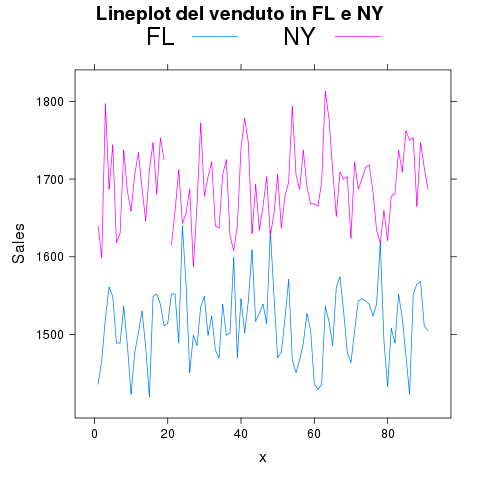
\includegraphics[width=7cm]{14_3.png}
	\end{center}
\begin{footnotesize}There are no relationship between the postcards sold in New York and in Florida.
\end{footnotesize}\end{frame}

%%%%%%%%%%%%%%%%%%%%%%%%%%%%%%%%%%%%%%%%%%%%%%%%%%%%%%%%%%%%%%%
\begin{frame} 
	\begin{center}
		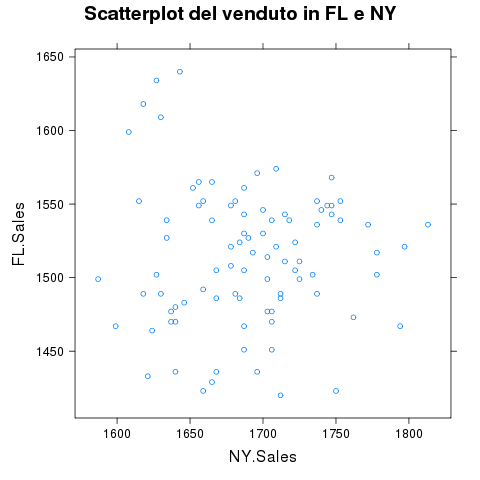
\includegraphics[width=7cm]{14_4.png}
	\end{center}
\begin{footnotesize}There are no relationship between the postcards sold in New York and in Florida.
\end{footnotesize}\end{frame}

%%%%%%%%%%%%%%%%%%%%%%%%%%%%%%%%%%%%%%%%%%%%%%%%%%%%%%%%%%%%%%%
\livelloB{Comparison between an adjusted and a non adjusted productive process}

%%%%%%%%%%%%%%%%%%%%%%%%%%%%%%%%%%%%%%%%%%%%%%%%%%%%%%%%%%%%%%%
\begin{frame} 
\begin{description}
	\item[Data:] adjust.txt\\
	Monitoring data of two production processes equal but one constantly monitored, while the other not.
	\item[Aims:] \begin{itemize}
				\item Let us numerically and graphically evaluate if It is better to monitor the processes knowing that, for the parameter analysed, the technically acceptable values must fall between 1,485 and 1,515, with central value in 1.5. 
				\begin{itemize}
					\item[-] Which are the main statistics of the two processes?
					\item[-] Which process is better? 
					\item[-] Why? 
					\item[-] What is the difference in performance of the two processes?
				\end{itemize}
				\item Let us do numerical and graphical analysis.
	                  \end{itemize}
\end{description}
\end{frame}

%%%%%%%%%%%%%%%%%%%%%%%%%%%%%%%%%%%%%%%%%%%%%%%%%%%%%%%%%%%%%%%
\begin{frame}
Computation of descriptive statistics and B-W graphic:
	\vspace{.3cm}
	\begin{footnotesize}
	\begin{tabular}{|l|rrrrrrr|}
	\hline
	& \textbf{Min}. & 1\textbf{st.Qu}. & \textbf{Median} & \textbf{Mean} & \textbf{3rd.Qu.} & \textbf{Max.} & \textbf{Sd}\\
	\hline
	\textbf{Adjust (N=50)} & 1.475 & 1.492 & 1.499 & 1.500 & 1.509 & 1.525 & 0.0128\\
	\textbf{NoAdjust (N=50)} & 1.480 & 1.495  & 1.499 & 1.498 & 1.504 & 1.509 & 0.0070\\
	\hline	
	\end{tabular}
	\end{footnotesize}
	\begin{center}
		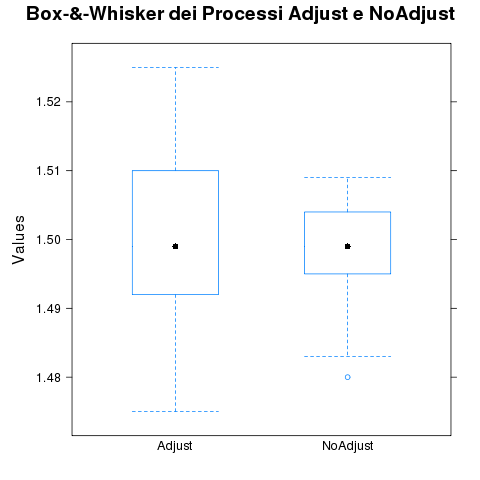
\includegraphics[width=6cm]{14_5.png}
	\end{center}
\end{frame}

%%%%%%%%%%%%%%%%%%%%%%%%%%%%%%%%%%%%%%%%%%%%%%%%%%%%%%%%%%%%%%%
\begin{frame}
	\begin{center}
		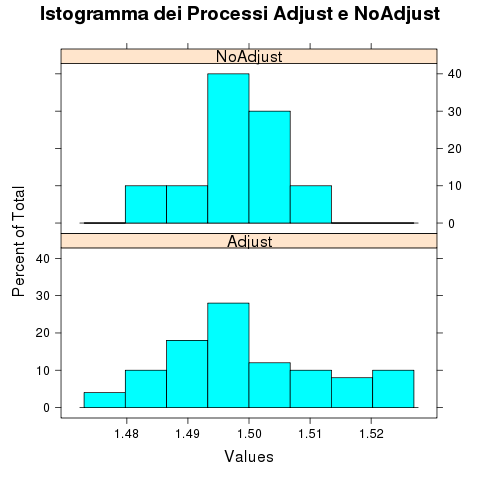
\includegraphics[width=7cm]{14_6.png}
	\end{center}
  \begin{center}  
\begin{footnotesize}Histograms illustrating the distribution of the data for the two processes.
\end{footnotesize}
  \end{center}
\end{frame}

%%%%%%%%%%%%%%%%%%%%%%%%%%%%%%%%%%%%%%%%%%%%%%%%%%%%%%%%%%%%%%%
\begin{frame}
  \begin{itemize}
    \item Data of both processes are centered around the central value of  technical acceptability.
    \item Both processes have a symmetrical distribution around the center. 
    \item The adjusted process seems to have a greater variability than the non adjusted process.
  \end{itemize}
\end{frame}

%%%%%%%%%%%%%%%%%%%%%%%%%%%%%%%%%%%%%%%%%%%%%%%%%%%%%%%%%%%%%%%
\begin{frame}
	\begin{center}
		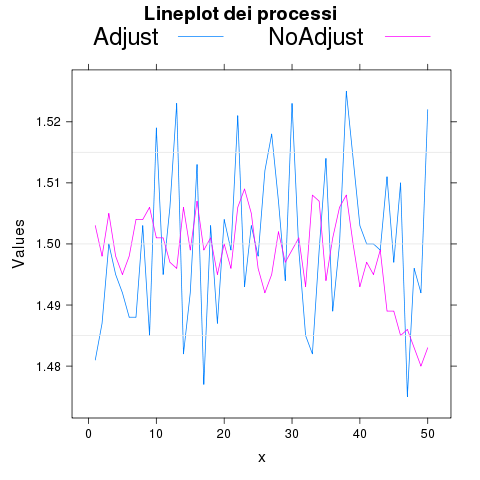
\includegraphics[width=7cm]{14_7.png}
	\end{center}
\begin{center}  
\begin{footnotesize} The adjusted process is more variable. The non adjusted process seems to ``go to drift'' downward in the last measurements.
\end{footnotesize}
  \end{center}
\end{frame}

%%%%%%%%%%%%%%%%%%%%%%%%%%%%%%%%%%%%%%%%%%%%%%%%%%%%%%%%%%%%%%%
\begin{frame}
  \begin{itemize}
    \item If you try to see how many times you have had out of specification values for each of the two processes, you obtain the following tables:
  \end{itemize}
  \begin{center}
    \begin{tabular}{|l|rr|c|l|rr|}
      \hline	
      \textbf{AdjustIn} & \textbf{No} & \textbf{S\`i} & & \textbf{NoAdjustIn} &  \textbf{No} & \textbf{S\`i} \\
      \hline
      \textbf{Counts} & 12 & 38 & & \textbf{Counts} & 3 & 47 \\
      \textbf{\%} & 24\% & 76\% & & \textbf{\%} & 6\% & 94\% \\
      \hline
    \end{tabular} 
  \end{center}
  \begin{itemize}
    \item It is evident how the non continuous adjusted processes generates a better final product, because It is more within specifications.
    \item Probably the continuous intervention of the operator in turn induces constant shifts in the average value of the process, increasing the variability to the process itself.
    \item The adjusted process produces significantly fewer pieces out of specification, as shown later (see the part relative to hypothesis testing).
  \end{itemize}
\end{frame}

%%%%%%%%%%%%%%%%%%%%%%%%%%%%%%%%%%%%%%%%%%%%%%%%%%%%%%%%%%%%%%%
\livelloB{Bond Strength Analysis}

%%%%%%%%%%%%%%%%%%%%%%%%%%%%%%%%%%%%%%%%%%%%%%%%%%%%%%%%%%%%%%%
\begin{frame} 
 
\begin{description}
	\item[Data:] bondstrength.txt\\
  Comparison data of the bond strenght of different formualtions of glues over time.
	\item[Aims:] \begin{itemize}
				\item Data of the strength necessary to separate two bonded surfaces with 6 different formulations of adhesive at a distance of 3, 6, 9 months is detected. 
				\begin{itemize}
					\item[-] Let us compare the holding of the 6 formulations.
					\item[-] Are there different variabilities in the 6 formulations?
					\item[-] Check if the holding decreases over time.
					\item[-] What are the formulations that satify the minimum requirement of holding 50 kg?
				\end{itemize}
				\item Let us do numerical and graphical analysis.
	                  \end{itemize}
\end{description}
 
\end{frame}

%%%%%%%%%%%%%%%%%%%%%%%%%%%%%%%%%%%%%%%%%%%%%%%%%%%%%%%%%%%%%%%
\begin{frame}
Computation of descriptive statistics and B-W graphic:\\
	\vspace{.3cm}
	\begin{footnotesize}
	\begin{tabular}{|l|rrrrrrr|}
	\hline
	& \textbf{Min}. & 1\textbf{st.Qu}. & \textbf{Median} & \textbf{Mean} & \textbf{3rd.Qu.} & \textbf{Max.} & \textbf{Sd}\\
	\hline
	\textbf{1+1 A} (N=72)& 43.00& 50.20& 53.50& 53.62& 57.50& 62.40& 4.34\\
	\textbf{1+1 B} (N=72)& 56.20& 64.00& 67.55& 67.23& 70.95& 74.60& 3.98\\
	\textbf{1+1 W} (N=72)& 47.90& 53.15& 54.80& 55.07& 56.97& 64.70& 3.19\\
	\textbf{2+2 B} (N=72)& 56.50& 63.82& 66.60& 66.27& 68.48& 77.70& 4.34\\
	\textbf{SS}    (N=72)& 25.90& 35.18& 40.55& 39.47& 44.05& 58.00& 6.24\\
	\textbf{XF}    (N=72)& 25.60& 33.65& 37.45& 37.83& 41.78& 56.00& 6.55\\
	\hline	
	\end{tabular}
	\end{footnotesize}
	\begin{center}
		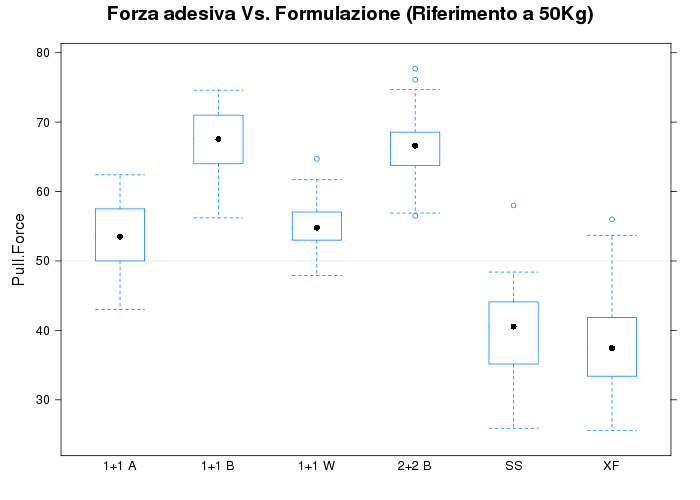
\includegraphics[width=6cm]{14_8.png}
	\end{center}
\end{frame}

%%%%%%%%%%%%%%%%%%%%%%%%%%%%%%%%%%%%%%%%%%%%%%%%%%%%%%%%%%%%%%%
\begin{frame}
\begin{itemize}
 \item It seems that the formulations with better holding are those characterized by the code \textbf{B}.
 \item The formulation with greater mean and median holding is \textbf{1+1 B}.
 \item The formualtions with lesser holding are \textbf{SS} and \textbf{XF}. These formulations have also a greater variability.
 \item The formulations \textbf{A} and \textbf{W} seem to have a non evedently higher variability than  \textbf{B}.
 \item The formulation \textbf{1+1 W} is the one with lesser variability.
 \item All the formulations present a distribution of the strength of separation approximately symmetrical.  
 \item The formulations that certainly satisfy the 50kg criterion, at least for the observed data, are \textbf{1+1 B} and  \textbf{2+2 B}. 
 \end{itemize}

\end{frame}

%%%%%%%%%%%%%%%%%%%%%%%%%%%%%%%%%%%%%%%%%%%%%%%%%%%%%%%%%%%%%%%
\begin{frame}
	\vspace{.3cm}
	\begin{center}
		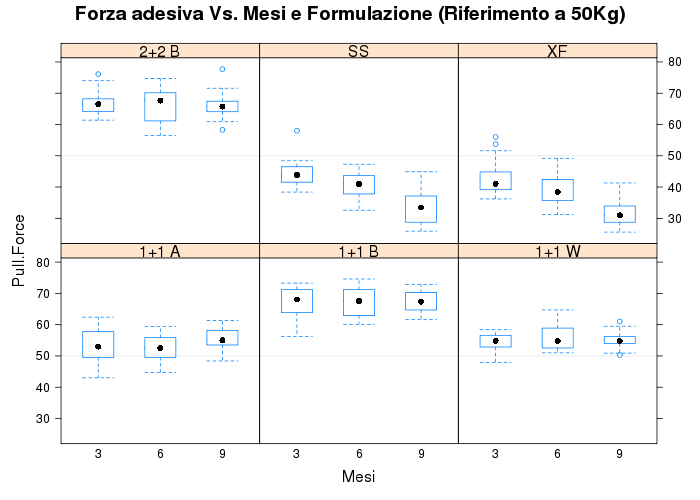
\includegraphics[width=9cm]{14_9.png}
	\end{center}
    \begin{center}
\begin{footnotesize}
 Description of the separation strength of the different formulations of glue varying the months (reference line: 50Kg). 
\end{footnotesize}
  \end{center}
\end{frame}

%%%%%%%%%%%%%%%%%%%%%%%%%%%%%%%%%%%%%%%%%%%%%%%%%%%%%%%%%%%%%%%
\begin{frame}
\begin{itemize}
 \item The impression given by the analysis of the formulations are confirmed.
 \item Over time, the bond strength decreases for the worst formulations. 
 \item The formulations with greater holding highligth a certain stability over time.
 \end{itemize}
\end{frame}



\livelloA{Correlation}

\livelloB{Mean diameter of caps produced by a forging machine}

\begin{frame} 
 
\begin{description}
	\item[Data:] bottlecap.txt\\
	\item[Aims:] Data of the mean diameter of the caps produced by a forging machine (let us see the following picture).
 Let us check if the caps diameter measures are correlated, so that It is possible to non measure all tha caps produced by the same machine in quality control phase.
				\begin{itemize}\begin{footnotesize}
					\item[-] Let us compute the main descriptive statistics for each cavity. 
					\item[-] Let us compute the correlations between the measures of cavities.
					\item[-] Let us graphically represent the diameter values between the pairs of cavities.
					\item[-] Is there very related cavities, enough to be ``replaceable'' in the measurements?  
				\end{footnotesize}\end{itemize}

\end{description}
 
\end{frame}

%%%%%%%%%%%%%%%%%%%%%%%%%%%%%%%%%%%%%%%%%%%%%%%%%%%%%%%%%%%%%%%
\begin{frame}
Scheme of the mould of caps:
\vspace{.3cm}
	\begin{center}
		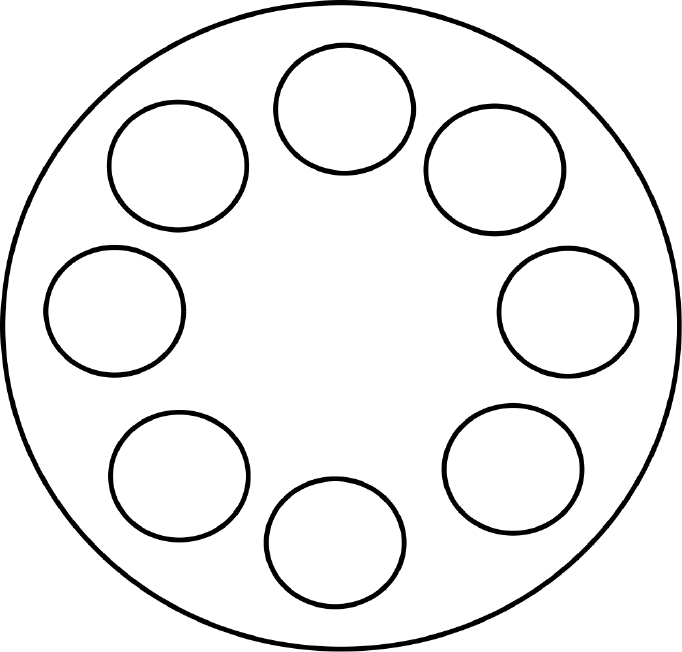
\includegraphics[width=6cm]{14_20.png}
	\end{center}
\end{frame}

%%%%%%%%%%%%%%%%%%%%%%%%%%%%%%%%%%%%%%%%%%%%%%%%%%%%%%%%%%%%%%%
\begin{frame}
Correlation matrix:\\
\vspace{.3cm}
\begin{tiny}
\begin{tabular}{l|rrrrrrrr}
         & Cavity.1 & Cavity.2 & Cavity.3 & Cavity.4 & Cavity.5 & Cavity.6 & Cavity.7 & Cavity.8\\
\hline
Cavity.1    & 1.000    & 0.858    & 0.650   & 0.459    & 0.193   & -0.115   & -0.037    & 0.343\\
Cavity.2    & 0.858    & 1.000    & 0.869    & 0.698    & 0.490    & 0.337   & 0.344    & 0.685\\
Cavity.3    & 0.650    & 0.869    & 1.000    & 0.604    & 0.471    & 0.401    & 0.399    & 0.601\\
Cavity.4    & 0.459    & 0.698    & 0.604    & 1.000    & 0.778    & 0.583    & 0.327    & 0.629\\
Cavity.5    & 0.193    & 0.490    & 0.471    & 0.778    & 1.000    & 0.627    & 0.417    & 0.627\\
Cavity.6   & -0.115    & 0.337    & 0.401    & 0.583    & 0.627    & 1.000    & 0.847    & 0.747\\
Cavity.7   & -0.037    & 0.344    & 0.399    & 0.327    & 0.417    & 0.847    & 1.000    & 0.542\\
Cavity.8    & 0.343    & 0.685    & 0.601    & 0.629    & 0.627    & 0.747    & 0.542    & 1.000\\
\end{tabular} 
\end{tiny}
\end{frame}

%%%%%%%%%%%%%%%%%%%%%%%%%%%%%%%%%%%%%%%%%%%%%%%%%%%%%%%%%%%%%%%
\begin{frame}
Scatterplot matrix of the relations between measures:
\vspace{.3cm}
	\begin{center}
		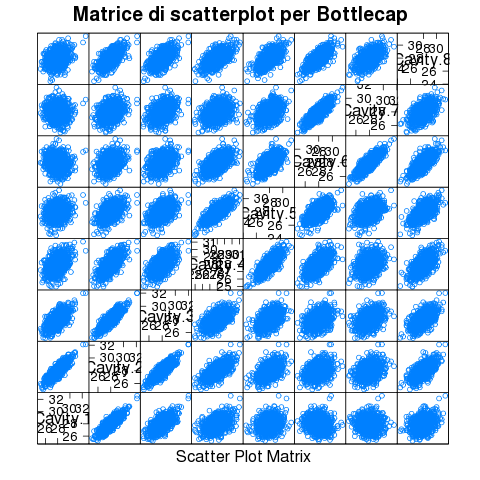
\includegraphics[width=7.5cm]{14_21.png}
	\end{center}
\end{frame}

%%%%%%%%%%%%%%%%%%%%%%%%%%%%%%%%%%%%%%%%%%%%%%%%%%%%%%%%%%%%%%%
\begin{frame}
\begin{itemize}
 \item Many of the measures have a high correlation value ($>.7$).
 \item In particular, the measures of Cavity.1 and Cavity.2, Cavity.2 and Cavity.3, Cavity.6 and Cavity.7 have a correlation value greater than .845. 
 \item Therefore the value of Cavity.2 instead of Cavity.1, or instead of Cavity.3 could be used.
 \item \textbf{Interesting note}: The correlations are not transitive: the correlation between Cavity.1 and Cavity.3 is .65, the correlation between Cavity.3 and Cavity.6 is .401; the correlation between Cavity.1 and Cavity.6 is negative! 
 \end{itemize}

\end{frame}


%%%%%%%%%%%%%%%%%%%%%%%%%%%%%%%%%%%%%%%%%%%%%%%%%%%%%%%%%%%%%%%
\livelloB{pH measure tools}
\begin{frame} 
 
\begin{description}
	\item[Data:] labtest.txt\\ 
	Comparison between the pH measure tools on the same samples of material.
	\item[Aims:] \begin{small}\begin{itemize}
				\item Let us check if the two tools (in lab and ``on the field'') give correlated values by measuring the same samples.
				\begin{itemize}
					\item[-] Let us compute the correlations between the measurements of the two equipments.
					\item[-] Let us graphically represent the diameter values between the pairs of measurements.
				\end{itemize}
	                  \end{itemize}
\end{small}
\end{description}
 
\end{frame}

%%%%%%%%%%%%%%%%%%%%%%%%%%%%%%%%%%%%%%%%%%%%%%%%%%%%%%%%%%%%%%%
\begin{frame}
Correlation matrix:\\
\vspace{.3cm}
\begin{footnotesize}
\begin{tabular}{l|rr}
 & Lab & Online\\
\hline
Lab & 1.000 & 0.959\\
Online & 0.959 & 1.000\\
\end{tabular} 
\end{footnotesize}

Scatterplot matrix of the relations between measures:
\vspace{.3cm}
	\begin{center}
		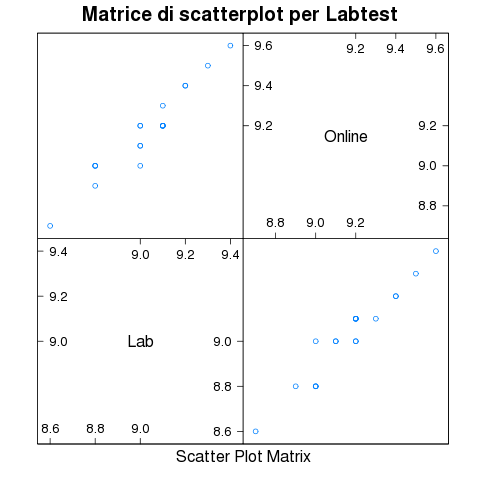
\includegraphics[width=5.5cm]{14_22.png}
	\end{center}
\end{frame}

%%%%%%%%%%%%%%%%%%%%%%%%%%%%%%%%%%%%%%%%%%%%%%%%%%%%%%%%%%%%%%%
\begin{frame}
Scatterplot della relazione con retta di regressione:\\
\vspace{.3cm}
	\begin{center}
		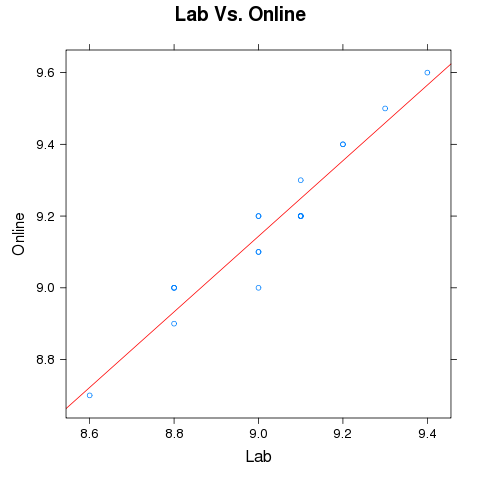
\includegraphics[width=6.5cm]{14_23.png}
	\end{center}
\end{frame}

%%%%%%%%%%%%%%%%%%%%%%%%%%%%%%%%%%%%%%%%%%%%%%%%%%%%%%%%%%%%%%%
\begin{frame}
\begin{itemize}
 \item The two measurements have a very high correlation value.  
 \item Considering the correlation, the two tools could be ``almost'' interchangeable. However, considering the previous analysis, which analyse the differences in pairs between the measured values, the on-line tool seems to produce values systematically different from the laboratory instrument.
 \end{itemize}

\end{frame}

